% layout.tex - 名刺レイアウト図(A4用紙)
\documentclass[tikz,border=3mm]{standalone}
\usepackage{tikz}
\usepackage{lmodern}

\begin{document}
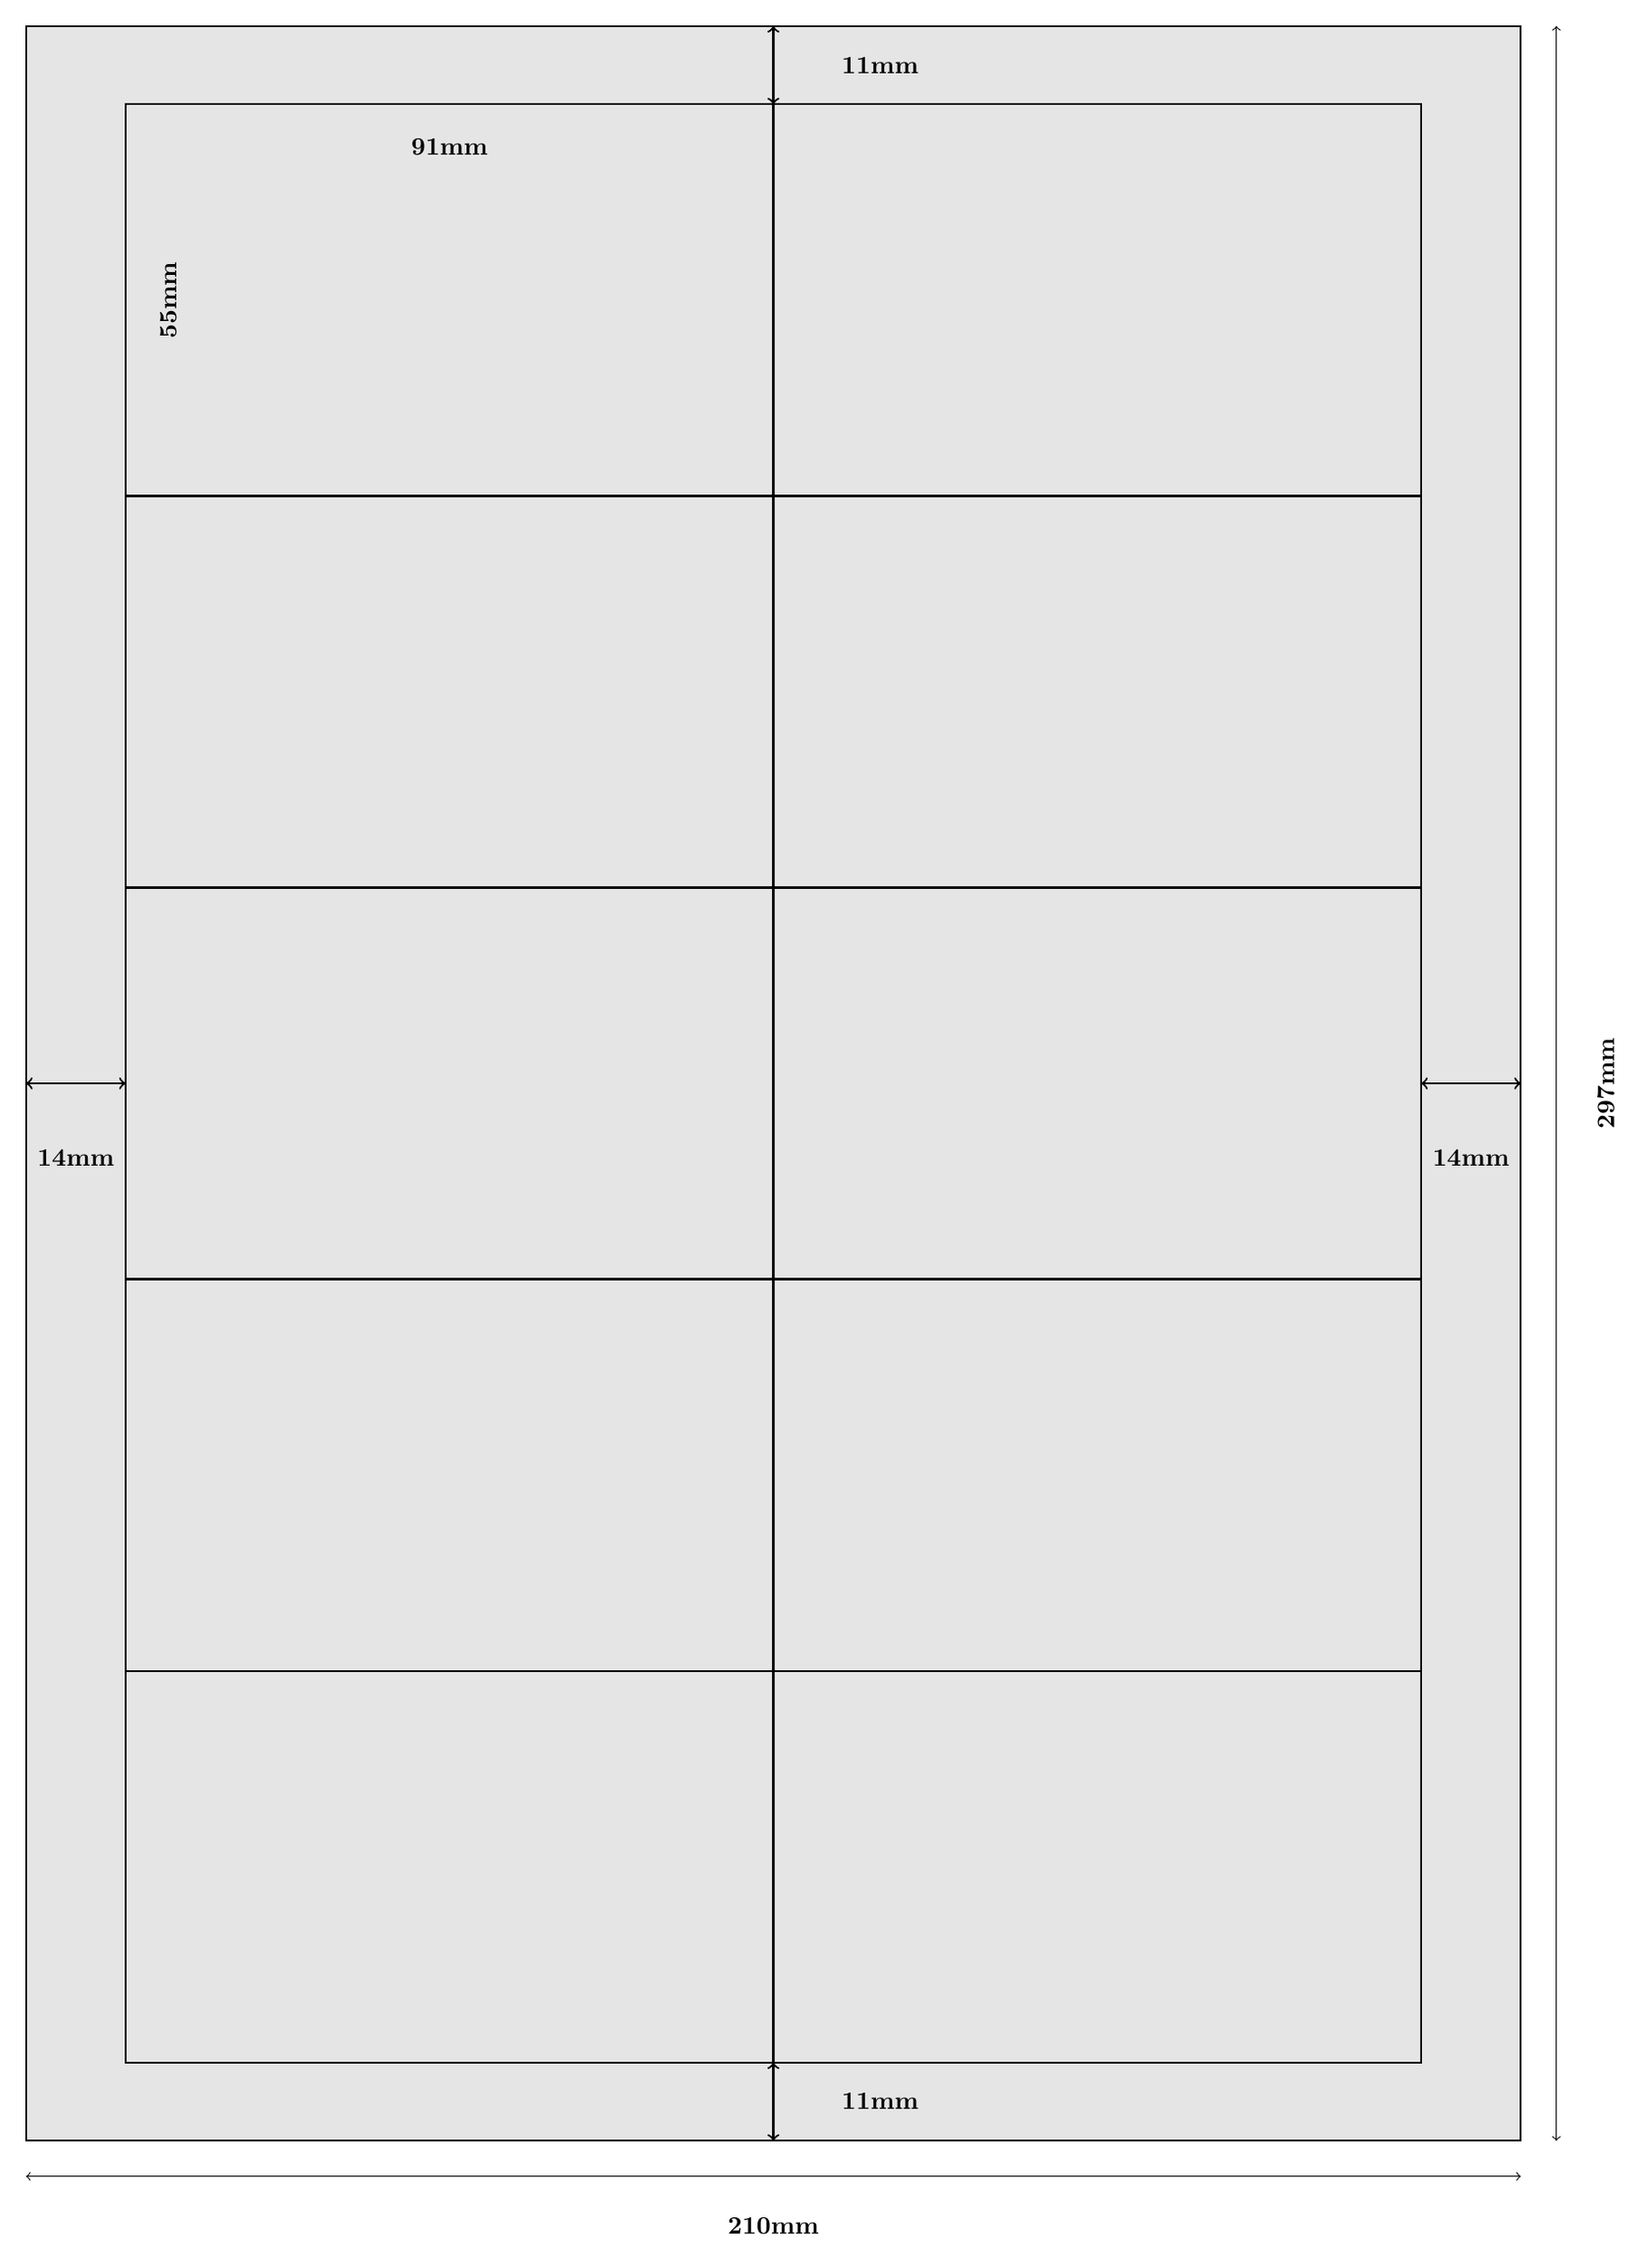
\begin{tikzpicture}[x=1mm, y=1mm, every node/.style={font=\normalsize}]
  % A4用紙の外枠 (210mm x 297mm) - 薄いグレー
  \draw[thick, fill=gray!20] (0,0) rectangle (210,297);

  % 名刺グリッド (2列×5行) - 紙と同じ色、黒い境界線
  \foreach \row in {0,1,2,3,4} {
    \foreach \col in {0,1} {
      \draw[fill=gray!20, draw=black, thick] (14+\col*91, 11+\row*55) rectangle (14+\col*91+91, 11+\row*55+55);
    }
  }

  % 用紙幅 (下)
  \draw[<->] (0,-5) -- (210,-5);
  \node at (105,-12) {\textbf{210mm}};

  % 用紙高さ (右)
  \draw[<->] (215,0) -- (215,297);
  \node[rotate=90] at (222,148.5) {\textbf{297mm}};

  % 左余白 (14mm) - 紙面内側に矢印
  \draw[<->, thick] (0,148.5) -- (14,148.5);
  \node at (7,138) {\textbf{14mm}};

  % 右余白 (14mm) - 紙面内側に矢印
  \draw[<->, thick] (196,148.5) -- (210,148.5);
  \node at (203,138) {\textbf{14mm}};

  % 上余白 (11mm) - 紙面内側に矢印
  \draw[<->, thick] (105,286) -- (105,297);
  \node at (120,291.5) {\textbf{11mm}};

  % 下余白 (11mm) - 紙面内側に矢印
  \draw[<->, thick] (105,0) -- (105,11);
  \node at (120,5.5) {\textbf{11mm}};

  % 名刺サイズ - カード内側、辺に沿って表示
  % 1行目左のカード
  \node at (59.5,280) {\textbf{91mm}};  % 上辺に沿って内側
  \node[rotate=90] at (20,258.5) {\textbf{55mm}};  % 左辺に沿って内側

\end{tikzpicture}
\end{document}
